\documentclass[]{article}
\usepackage{amsmath}
\usepackage{graphicx}
%\usepackage{xcolor}
\usepackage{hyperref}
\usepackage[dvipsnames]{xcolor}
\usepackage{matlab-prettifier}
\usepackage{array}
\usepackage{amsthm}
\usepackage{fullpage}

 \theoremstyle{theorem}
\newtheorem{structure}{Structure}%[section]


\graphicspath{ {images/} }
\usepackage{comment}

\setlength\parindent{0pt}

\title{Report: V{\small I}LMA}
\author{Jesus Miguel Adrian Matos}
\date{\today}


\begin{document}
\maketitle

\begin{abstract} 
\noindent This report is based on the seminar entitled {\it Visual grounding of verbs and nominalisations in multimodal models}, taken by Albert Gatt on May 29, 2024.
In particular, I focus my attention on explaining the \textbf{VILMA} functionalities: I will not mention what datasets the \textbf{VILMA} tests ware made on, but rather I will explain how it selects the foil-caption to carry out the tests. The report is structured as follows:

\textbf{Previous concepts:} concepts that are used in the report.

\textbf{Video Language Model Assessment:} I list models that will be evaluated by VILMA and I explain the VILMA tests.

\textbf{Pretrained models:} I list models evaluated by VILMA.

\textbf{Conclusions:} I observe several models on which the VILMA tests were applied, and I give a conclusion on VILMA benchmarks.




\end{abstract}

%\newpage 

\section{Previous concepts:}

\subsection{Image-Language models(IMLs):}
\noindent An image-language model is an artificial intelligence system designed to process and understand both visual and textual data, integrating these two modalities to perform various tasks. These models can generate text descriptions from images, produce images from text descriptions, and understand the relationships between visual and textual elements. Key capabilities and applications of image-language models include:

\begin{itemize}
\item \textbf{Image Captioning:} Generating descriptive text for a given image.
\item \textbf{Visual Question Answering (VQA):} Answering questions related to the content of an image.
\item \textbf{Image Generation from Text:} Creating images based on textual descriptions.
\item \textbf{Cross-modal Retrieval:} Finding images that match a given text or vice versa.
\item \textbf{Image-Text Matching:} Evaluating the relevance or similarity between an image and a text description.
\end{itemize}

\noindent These models typically combine techniques from computer vision (for processing videos) and natural language processing (for handling text). They often use deep learning architectures such as:

\begin{itemize}
\item \textbf{Convolutional Neural Networks (CNNs):} For extracting features from images.
\item \textbf{Transformers:} For handling and generating text, and sometimes for processing image features.
\item \textbf{Multimodal Models:} Like CLIP (Contrastive Language–Image Pretraining) and DALL-E, developed by OpenAI, which are specifically designed to understand and generate both images and text.
\end{itemize}
\subsection{Video-Language models(VidLMs):}
\noindent Video-language models are advanced machine learning systems designed to understand and generate both video content and associated natural language descriptions. These models can interpret and generate content involving the complex interplay between visual data (videos) and textual data (language). Key capabilities and applications of video-language models:

\begin{itemize}
\item \textbf{Video Captioning:} Automatically generating descriptive text for video content.
\item \textbf{Video Question Answering (Video QA):} Answering questions based on the content of a video.
\item \textbf{Text-to-Video Generation:} Creating video sequences from textual descriptions.
\item \textbf{Video Retrieval:} Finding relevant videos based on textual queries or descriptions.
\item \textbf{Action Recognition:} Identifying and classifying actions depicted in video clips.
\end{itemize}

\noindent These models typically combine techniques from computer vision (for processing videos) and natural language processing (for handling text). Here, there are some Architecture and Models:

\begin{itemize}
\item \textbf{Encoder-Decoder Frameworks:} Commonly used where the encoder processes video frames to create a rich representation and the decoder generates the corresponding textual description.
\item \textbf{Transformer-based Models:} These models leverage attention mechanisms to handle the complexity of video and language data, such as the Vision Transformer (ViT) and variants like VideoBERT.
\item \textbf{Fusion Techniques:} Methods to effectively combine and align visual and textual data, such as cross-modal attention and joint embedding spaces.
\end{itemize}
\section{Video Language Model Assessment(ViLMA):}

Es un benchmark independiente de la tarea que detalla evaluacion de las capacidades de los modelos(VidLMs) sobre una base firme.

Atravez de countrafactuales cuidadosamente selectionados, VILMA ofrece un conjunto de evaluciones controladas que arrojan luz sobre el verdadero potencial de estos modelos(VidLMs).

mientras tales evaluaciones arrojan luz sobre tareas de rendimiento y soporte para analisis coperativo, estos estan limitados a sus habilidades para revelar las capacidades visiolinguisticas que los modelos exiben a lo largo de las tareas.

\textbf{Comun estructura para cada test:}
\begin{enumerate}
\item In step 1, be harvested high-quality examples from existing \textbf{video-language datasets}.
\item In step 2, 
\end{enumerate}
\subsection{Pretrained VidLMs:}
Models used in this benchmark of VILMA.
\textbf{Unimodel Models:}
Modelos basados en solo texto (i.e. text-only MLs), tenemos 2 tipos:

decoder-only models: estos se enfocan en generar y predecir aspectos de tareas del lenguage como modelado del lenguaje, completacion de texto y generacion de texto, para los benchamarks se tiene:
\begin{itemize}
\item GPT2-2
\end{itemize}
Encoder-decoder models:Estos son los mismos que sequence-to-sequence, estos modelos procesan como input una sequencia a la cual se le debe asignar otra sequencia como respuesta, como por ejemplo traducion, resumir un texto y responder preguntas, para los benchmark se tiene:
\begin{itemize}
\item T5
\item BART
\item BOTH
\end{itemize}
and for both:
\begin{itemize}
\item OPT
\end{itemize}
Al igual que VALSE se calcula los perplexity values para ambos caption y foil, y tomamos el text intput con menor perpelxiti escore.
Parametros usados:
\begin{itemize}
\item GPT-2 124M
\item OPT 6.7B
\end{itemize}


\textbf{Image Language Models:}
La definicion de una Image Language model se encuentra en la subsecion \ref{ilm}.
Los modelos usados para los benchmarks son:
\begin{itemize}
\item CLIP
\item BLIP
\end{itemize}
Ambos con OPT model.
 
\textbf{Video Language Models:}
La definicion de Video Lnaguage Model se encuentra subsection \ref{vlm}.
Listado de Modelos usados pata benchmark:
\begin{itemize}
\item ClipBERT:
\begin{itemize}
\item Text-encoder: BERT
\item Video-encoder: Resnet-50
\item Features:
\begin{enumerate}
\item Este pretrainet usa solamente imagenes.
\item No aprende orden temporal: El escore de similitud de Video-text es el promedio de el escore de similitud de frame-text.
\end{enumerate}
\end{itemize}
\end{itemize}

\begin{itemize}
\item UniVL:
\begin{itemize}
\item Text-encoder: BERT
\item Video-encoder: S3D
\item Features:
\begin{enumerate}
\item Dual-stream Architecture: UniVL employs a dual-stream architecture consisting of a video encoder and a text encoder. The video encoder processes the visual information, while the text encoder processes the language information. Both encoders are built using Transformer layers.
\item Cross-modal Transformer: After encoding the video and text separately, UniVL employs a cross-modal Transformer to fuse the information from both modalities. This cross-modal Transformer is crucial for understanding and generating coherent video-language representations.
\item UniVL is pretrained on HowTo100M.
\end{enumerate}
\end{itemize}
\end{itemize}

\begin{itemize}
\item VideoCLIP:
\begin{itemize}
\item Text-encoder: BERT
\item Video-encoder: S3D
\item Features:
\begin{enumerate}
\item it uses mean pooling to fuse modalities, this is similar to the Video-text similarity score for ClipBERT.
\item VideoCLIP is pretrained on HowTo100M.
\end{enumerate}
\end{itemize}
\end{itemize}

\begin{itemize}
\item FiT:
\begin{itemize}
\item Text-encoder: BERT
\item Video-encoder: TimeSFormer
\item Features:
\begin{enumerate}
\item it be able to be pretrained on images(CC3M) and videos(W2).
\item it creates a shared video-text space through contrastive learning. 
\end{enumerate}
\end{itemize}
\end{itemize}

\begin{itemize}
\item CLIP4Clip:
\begin{itemize}
\item Text-encoder: BERT
\item Video-encoder: Resnet-50
\item Features:
\begin{enumerate}
\item Its primary goal is to enable effective retrieval of videos based on textual descriptions and vice versa. 
\item Video Representation: It uses the Clip video encoder, processing each frame as if it were an image.
\item Text Representation: It use the Clip text encoder. Textual queries or descriptions are encoded into embeddings that reside in the same space as the video frame embeddings.
\item Strategy for modeling space-time:
\begin{itemize}
\item Simple aggregation methods like mean pooling over frame embeddings.
\item Sophisticated techniques such as attention mechanisms to capture the temporal dependencies between frames.
\end{itemize}
\end{enumerate}
\end{itemize}
\end{itemize}

\begin{itemize}
\item 	VIOLET:
\begin{itemize}
\item Text-encoder: BERT
\item Video-encoder: Video Swin Transformer
\item Features:
\begin{enumerate}
\item it be able to be pretrained on images(CC3M) and videos(YT-Temporal, WebVid).
\item Spatial and temporal dimensions of the video inputs are modelled by positional embeddings considering both spatial and temporal ordering. 
\end{enumerate}
\end{itemize}
\end{itemize}

\begin{itemize}
\item 	X-Clip:
\begin{itemize}
\item Text-encoder: BERT
\item Video-encoder: Resnet-50, or ViT
\item Features:
\begin{enumerate}
\item Contrastive Loss: During training, the model uses a contrastive loss function, typically a variant of the InfoNCE (Information Noise Contrastive Estimation) loss. This loss encourages the similarity scores of matching video-text pairs to be higher than those of non-matching pairs.
\item It introduces the Attention Over Similarity Matrix (AOSM) module, enabling it to focus on essential frames and words while reducing the impact of irrelevant ones during retrieval.
\end{enumerate}
\end{itemize}
\end{itemize}

MCQ(Definition in section\ref{mcq_model}): A pretext task using Multiple Choice Questions (MCQ) was introduced for video-text pretraining, utilizing a dual-encoder approach. This involved a parametric module named BridgeFormer, which links local features from both VideoFormer and TextFormer to address multiple-choice questions through a contrastive learning objective. This method enhances the semantic connections between video and text representations, improving detailed semantic associations between the two modalities. Furthermore, it ensures high efficiency for retrieval, and the BridgeFormer can be omitted for downstream tasks.

\begin{itemize}
\item Singularity:
\begin{itemize}
\item Text-encoder: BERT
\item Video-encoder: ViT
\item Features:
\begin{enumerate}
\item In the training phase, a single frame is randomly selected as input, and a video-level prediction is made using the information from this frame and its corresponding text input. During inference, multiple frames are uniformly sampled, and their encoded image-level representations are combined early on as input to the multi-modal encoder, see Figure \ref{fig:singularity_m}.
\end{enumerate}
\end{itemize}
\end{itemize}

\begin{figure}[h]
    \centering
    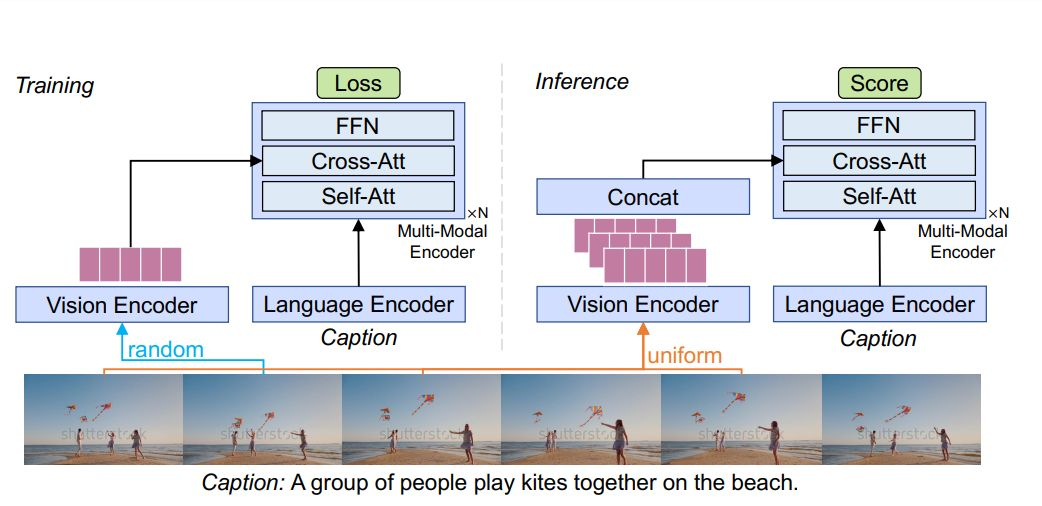
\includegraphics[width=0.55\textwidth]{singularity_model}
    \caption{Process of the Singularity model}
    \label{fig:singularity_m}
\end{figure}

UniPerceiver: It is used for perception tasks in videos. The model is designed to handle zero-shot and few-shot learning situations. UniPerceiver was inspired by the Transformer architecture but uses CNN for a variety of modalities such as text, images and videos. See Figure \ref{fig:uniPerceiver_m}

\begin{figure}[h]
    \centering
    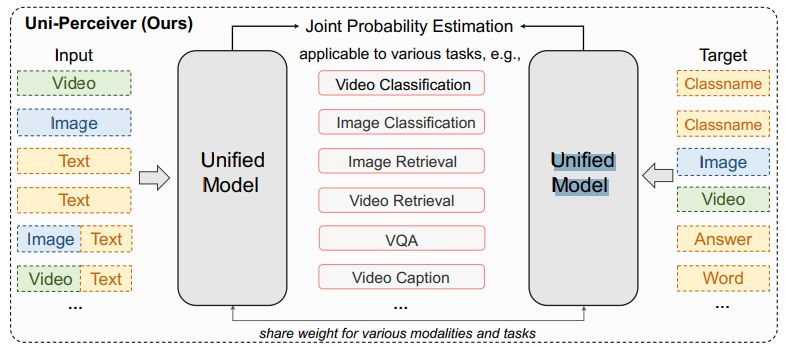
\includegraphics[width=0.55\textwidth]{uniPerceiver_model}
    \caption{Process of the UniPerceiver model}
    \label{fig:uniPerceiver_m}
\end{figure}

Merlot Reserve: It has a better understanding of temporal space for videos by combining audio, subtitles, and video frames. The model learns by substituting bits of text and audio with a MASK token and selecting the one that fits best describes the image. 

\begin{itemize}
\item VindLU:
\begin{itemize}
\item Text-encoder: BERT
\item Video-encoder: BEiT (BERT Pre-Training of image transformer)
\item Features:
\begin{enumerate}
\item Use a visual-text contrastive objective.
\item These models add the following steps to improve their result: the inclusion of temporal attention, integration of a multimodal fusion encoder, adoption of masked modeling pretraining objectives, joint training on images and videos, utilization of additional frames both in fine-tuning and inference stages, model-parameter and data scaling.
\end{enumerate}
\end{itemize}
\end{itemize}
\section{conclusion:}

In Figure \ref{fig:test_model} we can see the scores of the \textbf{VILMA} tests, for various models, where the letters \textbf{P} represent the main test and the \textbf{T} represents the \textbf{Proficiency test}.

These are ordered as follows, the first 2 are the \textbf{simple LM}, the next 2 are the \textbf{ILM}, and the rest are the \textbf{VidLM}.

\textbf{Observations from figure 2:}

So we can notice that the best scores are for the Image Language Model (ILM), the VidLMs have score aceptable, and as it was waiting, the LM are the ones with the lowest score, because they do not have images to validate some tests.

We can also noted that simple LMs have good scores in proficiency tests, since these do not imply a strong spatio-temporal relations.
\begin{figure}[h]
    \centering
    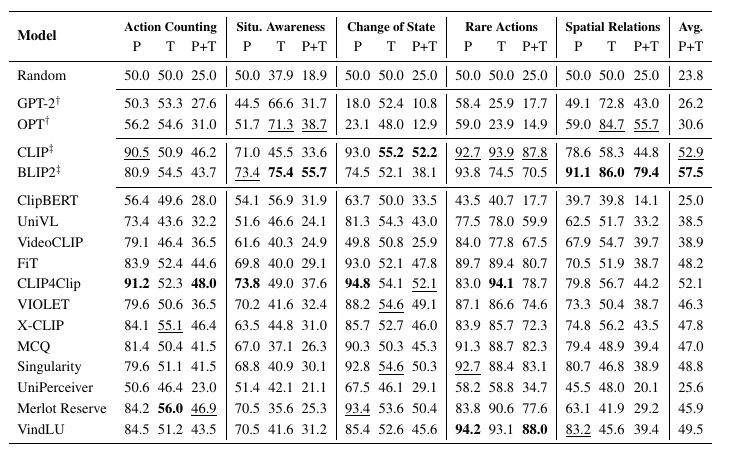
\includegraphics[width=0.25\textwidth]{test_model}
    \caption{Score of the models where the VILMA test was carried out}
    \label{fig:test_model}
\end{figure}

Therefore, I can conclud that VILMA is more focused on VidLM that has spatio-temporal relations for videos, and is also very good for ILM, since the frames of a video are images and VILMA uses a constant frequency of frames to carry out their tests, which allows us to have images that represent periods of frames, and with this method a video could be considered as a set of images but with a space-time relations.

\newpage
\begin{thebibliography}{}
    
\bibitem{lei2021clipbert}
J. Lei et al., "Less is More: CLIPBERT for Video-and-Language Learning via Sparse Sampling," 2021 IEEE/CVF Conference on Computer Vision and Pattern Recognition (CVPR), Nashville, TN, USA, 2021, pp. 7327-7337, doi: 10.1109/CVPR46437.2021.00725.

\bibitem{Buchen-Mainardi 1975}
P.W. Buchen, F. Mainardi,Asymptotic expansions for transient viscoelastic waves, {\it Journal de M{\'e}canique} {14},  597--608 (1975).

\bibitem{AG-FM_MECC16}
A. Giusti, F. Mainardi, A dynamic viscoelastic analogy for fluid-filled elastic tubes, {\it Mecanica}, published on line, 04 February  2016.(2015).
\end{thebibliography}

\end{document}          
